% Pengaturan ukuran teks dan bentuk halaman dua sisi
\documentclass[12pt]{book}

% Pengaturan ukuran halaman dan margin
\usepackage[a4paper,top=30mm,left=30mm,right=20mm,bottom=25mm]{geometry}

% Pengaturan ukuran spasi
\usepackage[singlespacing]{setspace}

% Pengaturan caption untuk tabel
\usepackage{caption}

% Judul dokumen
\title{Proposal Tugas Akhir ITS}
\author{Shadiq, Ja'far}

% Pengaturan detail pada file PDF
\usepackage[pdfauthor={\@author},bookmarksnumbered,pdfborder={0 0 0}]{hyperref}


% Pengaturan ukuran indentasi
\setlength{\parindent}{2em}

% Package lainnya
\usepackage{changepage}
\usepackage{etoolbox} % Mengubah fungsi default

% Pengaturan jenis karakter
\usepackage[utf8]{inputenc}

\usepackage[style=apa, backend=biber]{biblatex}
\usepackage{enumitem} % Pembuatan list
\usepackage{lipsum} % Pembuatan template kalimat
\usepackage{graphicx} % Input gambar
\usepackage{longtable} % Pembuatan tabel
\usepackage[table,xcdraw]{xcolor} % Pewarnaan tabel
\usepackage{eso-pic} % Untuk menggunakan background image di halaman
\usepackage{txfonts} % Font times
\usepackage{changepage} % Pembuatan teks kolom
\usepackage{multicol} % Pembuatan kolom ganda
\usepackage{multirow} % Pembuatan baris ganda
\usepackage{tabularx} % Untuk mengatur kolom, seperti grid pada CSS
\usepackage{wrapfig}
\usepackage{float}

% Pengaturan format daftar isi, daftar gambar, dan daftar tabel
\usepackage[titles]{tocloft}
\setlength{\cftsecindent}{2em}
\setlength{\cftsubsecindent}{2em}
\setlength{\cftbeforechapskip}{1.5ex}
\setlength{\cftbeforesecskip}{1.5ex}
\setlength{\cftbeforetoctitleskip}{0cm}
\setlength{\cftbeforeloftitleskip}{0cm}
\setlength{\cftbeforelottitleskip}{0cm}
\renewcommand{\cfttoctitlefont}{\hfill\Large\bfseries} % command untuk membuat heading bold dan besar
\renewcommand{\cftaftertoctitle}{\hfill}
\renewcommand{\cftloftitlefont}{\hfill\Large\bfseries}
\renewcommand{\cftafterloftitle}{\hfill}
\renewcommand{\cftlottitlefont}{\hfill\Large\bfseries}
\renewcommand{\cftafterlottitle}{\hfill}

% Definisi untuk "Hati ini sengaja dikosongkan"
\patchcmd{\cleardoublepage}{\hbox{}}{
  \thispagestyle{empty}
  \vspace*{\fill}
  \begin{center}\textit{[Halaman ini sengaja dikosongkan]}\end{center}
  \vfill}{}{}

  % Pengaturan penomoran halaman
\usepackage{fancyhdr}
\fancyhf{}
\renewcommand{\headrulewidth}{0pt}
\pagestyle{fancy}
\fancyfoot[C,CO]{\thepage}
\patchcmd{\chapter}{plain}{fancy}{}{}
\patchcmd{\chapter}{empty}{plain}{}{}

% Pengaturan format judul bab
\usepackage{titlesec}
\renewcommand{\thesection}{\thechapter.\arabic{section}}
\titleformat{\chapter}[hang]{\centering\bfseries\large}{BAB\ \arabic{chapter}\ }{0ex}{\vspace{0ex}\centering}
\titleformat*{\section}{\large\bfseries}
\titleformat*{\subsection}{\normalsize\bfseries}
\titlespacing{\chapter}{0ex}{0ex}{4ex}
\titlespacing{\section}{0ex}{1ex}{0ex}
\titlespacing{\subsection}{0ex}{0.5ex}{0ex}
\titlespacing{\subsubsection}{0ex}{0.5ex}{0ex}
\setcounter{secnumdepth}{3} % Untuk memberi penomoran pada \subsubsection

\counterwithin{figure}{chapter}
\counterwithin{table}{chapter}

% Mengganti figure dan table menjadi gambar dan tabel
\renewcommand{\figurename}{Gambar}
\renewcommand{\tablename}{Tabel}

% Tambahkan format tanda hubung yang benar di sini
\hyphenation{
  ro-ket
  me-ngem-bang-kan
  per-hi-tu-ngan
}

% Menambahkan resource daftar pustaka
\addbibresource{pustaka/pustaka.bib}

% Isi keseluruhan dokumen
\begin{document}
  % Nomor halaman pembuka dimulai dari sini
  \pagenumbering{roman}

  % Atur ulang penomoran halaman
  \setcounter{page}{1}

  % Sampul Bahasa Indonesia
  \newcommand\covercontents{sampul/konten-id.tex}
  \AddToShipoutPictureBG*{
  \AtPageLowerLeft{
    % Ubah nilai berikut jika posisi horizontal background tidak sesuai
    \hspace{-3.25mm}

    % Ubah nilai berikut jika posisi vertikal background tidak sesuai
    \raisebox{0mm}{
      
\includegraphics[width=\paperwidth,height=\paperheight]{sampul/gambar/sampul-luar-tipis.png}
    }
  }
}

% Menyembunyikan nomor halaman
\thispagestyle{empty}

% Pengaturan margin untuk menyesuaikan konten sampul
\newgeometry{
  top=65mm,
  left=30mm,
  right=30mm,
  bottom=20mm
}

\begin{flushleft}

  % Pemilihan font sans serif
  \sffamily

  % Pemilihan font bold
  \fontseries{bx}
  \selectfont
  \begin{spacing}{1.5}
    \input{\covercontents}
  \end{spacing}

\end{flushleft}

\restoregeometry


  % Lembar pengesahan
  \chapter*{LEMBAR PENGESAHAN}

% Menyembunyikan nomor halaman
\thispagestyle{empty}

\begin{center}
  % Ubah kalimat berikut dengan judul tugas akhir
  \textbf{Sistem Pemantauan Ketersediaan Ruangan pada Gedung Perkuliahan Berbasis Okupansi Menggunakan Kamera}
\end{center}

\begingroup
% Pemilihan font ukuran small
\small

\begin{center}
  % Ubah kalimat berikut dengan pernyataan untuk lembar pengesahan
  \textbf{PROPOSAL TUGAS AKHIR} \\
  Diajukan untuk memenuhi salah satu syarat memperoleh gelar
  Sarjana Teknik pada
  Program Studi S-1 Teknik Komputer \\
  Departemen Teknik Komputer \\
  Fakultas Teknologi Elektro dan Informatika Cerdas \\
  Institut Teknologi Sepuluh Nopember
\end{center}

\begin{center}
  % Ubah kalimat berikut dengan nama dan NRP mahasiswa
  Oleh: \textbf{Ja'far Shadiq} \\
  NRP. 0721 19 4000 0023
\end{center}

\begin{center}
  Disetujui Oleh:
\end{center}

\vspace{10ex}

\begingroup
% Menghilangkan padding
\setlength{\tabcolsep}{0pt}

\noindent
\begin{tabularx}{\textwidth}{X c}
  % Ubah kalimat-kalimat berikut dengan nama dan NIP dosen pembimbing pertama
  Dion Hayu Fandiantoro, S.T., M.T.      &                 \\
  NIP: 1994202011064    & (Pembimbing)    \\
                                &                 \\
                                &                 \\
                                &                 \\
  % Ubah kalimat-kalimat berikut dengan nama dan NIP dosen pembimbing kedua
  Eko Pramunanto, S.T., M.T. &                 \\
  NIP: 19661203199412 1 001    & (Ko-Pembimbing) \\
\end{tabularx}
\endgroup

\vspace{\fill}
\begin{center}
  % Ubah text dibawah menjadi tempat dan tanggal

  Mengetahui, \\
  Kepala Departemen Teknik Komputer FTEIC ITS \\
  \vspace{\fill}
  \underline{Dr. Supeno Mardi Susiki Nugroho, S.T., M.T.} \\
  197003131995121001
  
\end{center}

% \vspace{\fill}

\begin{center}
  % Ubah text dibawah menjadi tempat dan tanggal
  \textbf{SURABAYA} \\
  \textbf{Juni, 2023}
\end{center}
\endgroup

  \cleardoublepage

  % Abstrak
  \chapter*{ABSTRAK}
\begin{center}
  \large
  \textbf{Sistem Pemantauan Ketersediaan Ruangan pada Gedung Perkuliahan Berbasis Okupansi Menggunakan Kamera}
\end{center}
\addcontentsline{toc}{chapter}{ABSTRAK}
% Menyembunyikan nomor halaman
\thispagestyle{empty}

\begin{flushleft}
  \setlength{\tabcolsep}{0pt}
  \bfseries
  \begin{tabular}{ll@{\hspace{6pt}}l}
  Nama Mahasiswa / NRP&:& Ja'far Shadiq / 07211940000023\\
  Departemen&:& Teknik Komputer FTEIC - ITS\\
  Dosen Pembimbing&:& 1. Dion Hayu Fandiantoro, S.T., M.T..\\
  & & 2. Eko Pramunanto, S.T., M.T.\\
  \end{tabular}
  \vspace{4ex}
\end{flushleft}
\textbf{Abstrak}

% Isi Abstrak
Teknologi informasi yang ada saat ini berkembang pesat, dan dapat menawarkan peningkatan efisiensi di berbagai bidang. Dalam lingkup smart building, peningkatan efisiensi yang memungkinkan diantaranya kemudahan manajemen, penghematan biaya, peningkatan kelestarian lingkungan, dan lainnya. Penelitian ini bertujuan untuk mengetahui cara mendeteksi okupansi, dan mengembangkan alat yang dapat mendeteksi ketersediaan ruang berdasarkan okupansi menggunakan kamera. Sistem ini akan dilengkapi dengan teknologi deep learning, sehingga kamera dapat mendeteksi ada tidaknya orang dalam ruangan. Sistem ini diharapkan dapat dipasang di gedung perkuliahan atau kantor dosen. Sistem ini berpotensi untuk meningkatkan optimalisasi penggunaan ruang yang efektif, penghematan biaya, peningkatan kelestarian lingkungan, dan lainnya.

\vspace{2ex}
\noindent
\textbf{Kata Kunci: \emph{Internet of Things, Okupansi, Smart Building}}
  \cleardoublepage

  \chapter*{ABSTRACT}
\begin{center}
  \large
  \textbf{\emph{ANTI-GRAVITY} BASED ENERGY CALCULATION ON OUTER SPACE ROCKETS}
\end{center}
% Menyembunyikan nomor halaman
\thispagestyle{empty}

\begin{flushleft}
  \setlength{\tabcolsep}{0pt}
  \bfseries
  \begin{tabular}{lc@{\hspace{6pt}}l}
  Student Name / NRP&: &Ja'far Shadiq / 07211940000023\\
  Department&: &Computer engineering FTEIC - ITS\\
  Advisor&: &1. Dion Hayu Fandiantoro, S.T., M.T.\\
  & & 2. Eko Pramunanto, S.T., M.T.\\
  \end{tabular}
  \vspace{4ex}
\end{flushleft}
\textbf{Abstract}

% Isi Abstrak
Information technology that exists today is growing rapidly and can offer increased efficiency in various fields. Within the scope of smart building, possible efficiency improvements include ease of management, cost savings, increased environmental sustainability, and others. This study aims to find out how to detect occupancy and to develop a tool that can detect space availability based on occupancy using a camera. This system will be equipped with deep learning technology so that the camera can detect whether or not there are people in the room. This system is expected to be installed in lecture buildings or lecturer offices. This system has the potential to improve the optimization of effective use of space, cost savings, increased environmental sustainability, and others.

\vspace{2ex}
\noindent
\textbf{Keywords: \emph{Internet of Things, Occupancy, Smart Building}}
  \cleardoublepage

  \begin{spacing}{1.5}
    % Daftar isi
    \renewcommand*\contentsname{DAFTAR ISI}
    \addcontentsline{toc}{chapter}{\contentsname}
    \tableofcontents
    \cleardoublepage

    % Daftar gambar
    \renewcommand*\listfigurename{DAFTAR GAMBAR}
    \addcontentsline{toc}{chapter}{\listfigurename}
    \listoffigures
    \cleardoublepage

    % Daftar tabel
    \renewcommand*\listtablename{DAFTAR TABEL}
    \addcontentsline{toc}{chapter}{\listtablename}
    \listoftables
    \cleardoublepage
  \end{spacing}

  % Nomor halaman isi dimulai dari sini
  \pagenumbering{arabic}

  % Konten pendahuluan
  \chapter{PENDAHULUAN}

\section{Latar Belakang}

% Ubah paragraf-paragraf berikut sesuai dengan latar belakang dari tugas akhir
Teknologi informasi yang ada saat ini berkembang pesat, dan dapat menawarkan peningkatan efisiensi di berbagai bidang. Dalam lingkup smart building, peningkatan efisiensi yang memungkinkan diantaranya kemudahan manajemen, penghematan biaya, peningkatan kelestarian lingkungan, dan lainnya. Internet of things (IoT) adalah integrasi dari beberapa teknologi untuk menyediakan layanan cerdas (smart services) di lingkungan yang cerdas. IoT ini sangat mungkin untuk diterapkan di kampus untuk membantu kegiatan operasional.


Penerapan IoT di lingkungan kampus ini berkaitan dengan konsep ‘kampus cerdas’, dan ini dapat meningkatkan pengalaman belajar mahasiswa, keamanan kampus dan juga efisiensi operasional [1]. 
Salah satu penerapan yang memungkinkan dari sistem tersebut di universitas adalah untuk mendukung pengguna untuk menemukan ruang yang tersedia. Dengan sistem manajemen ruang yang optimal, penggunaan ruangan ini dilakukan dengan efisien dengan tujuan memaksimalkan penggunaan ruang sekaligus meminimalkan biaya operasi dan pemeliharaan. Optimalisasi penggunaan ruang ini juga mengarah langsung pada penghematan energi. Lebih lanjut lagi, informasi mengenai okupansi ini berguna untuk perencanaan strategis antara lain untuk mengidentifikasi permintaan untuk jenis ruang tertentu [2]. Ini dapat menjadi salah satu upaya untuk memaksimalkan pemanfaatan ruang kuliah yang efektif dengan modifikasi manajemen operasi yang ada. Di sisi lain, manajemen ruang yang optimal memungkinkan untuk menutup beberapa ruang kuliah sehingga mengurangi biaya sewa untuk universitas atau mengizinkan ruang kuliah untuk disewakan pihak luar untuk menghasilkan pendapatan tambahan bagi bangunan kampus yang ada [3]. 


\section{Rumusan Masalah}

% Ubah paragraf berikut sesuai dengan rumusan masalah dari tugas akhir
Berdasarkan latar belakang yang telah dipaparkan, rumusan masalah yang akan diselesaikan adalah bagaimana cara untuk mendeteksi okupansi, dan
bagaimana cara mengembangkan alat yang dapat mendeteksi ketersediaan ruang secara otomatis berdasarkan okupansi menggunakan kamera.


\section{Batasan Masalah atau Ruang Lingkup}

Ruang lingkup penelitian ini adalah penerapan IoT pada lingkungan kampus untuk mewujudkan {\it smart building}. Sistem yang dikembangkan menggunakan mikrokontroler, dan akan memggunakan kamera sebagai sensor untuk mendapatkan data citra.
Software dikembangkan hanya untuk sistem perhitungan, dan hanya sampai ke pengiriman hasil perhitungan.

\section{Tujuan}

% Ubah paragraf berikut sesuai dengan tujuan penelitian dari tugas akhir
Tujuan dari pembuatan tugas akhir ini adalah untuk mengetahui cara mendeteksi okupansi, dan mengembangkan alat yang dapat mendeteksi ketersediaan ruang secara otomatis berdasarkan okupansi menggunakan kamera. Produk jadi hasil perkembangan dibuat menggunakan komponen yang ekonomis, memiliki ukuran keseluruhan yang ringkas, dan  biaya keseluruhan yang ekonomis

\section{Manfaat}

% Ubah paragraf berikut sesuai dengan tujuan penelitian dari tugas akhir
% Manfaat dari penelitian ini adalah sebagai wadah penulis untuk mengembangkan dan mengimplementasikan keahlian penerapan IoT. Diharapkan pula penelitian ini berdampak pada Institut dimana perangkat ini dapat digunakan dalam ruang perkuliahan dan dapat bersaing dengan produk yang ditawarkan pihak ketiga.
  \cleardoublepage

  % Konten tinjauan pustaka
  \chapter{TINJAUAN PUSTAKA}

% Ubah konten-konten berikut sesuai dengan isi dari tinjauan pustaka
\section{Hasil penelitian/perancangan terdahulu}
Makalah "\emph{Experimental Evaluation of Internet of Things in the Educational Environment}" oleh Amr Elsaadany dan Mohamed Soliman mempelajari potensi manfaat dan dampak Internet of Things (IoT) di lingkungan pendidikan. Penulis berpendapat bahwa IoT memiliki potensi untuk merevolusi pendidikan dengan memberikan siswa pengalaman belajar yang dipersonalisasi, meningkatkan kolaborasi dan komunikasi, dan membuat pembelajaran lebih menarik dan interaktif.
Penulis melakukan evaluasi eksperimental IoT di lingkungan universitas. Mereka menggunakan berbagai perangkat IoT, termasuk sensor, aktuator, dan tag RFID, untuk mengumpulkan data tentang perilaku dan kinerja siswa. Data tersebut digunakan untuk mengembangkan model pembelajaran yang dipersonalisasi untuk setiap siswa. Model ini kemudian digunakan untuk memberi siswa umpan balik dan saran yang disesuaikan untuk perbaikan.

Rahman et al. (2020) dalam makalahnya menyajikan model pemanfaatan ruang untuk institusi pendidikan tinggi (PT). Model dikembangkan dengan wawancara dan diskusi kelompok terarah dengan pemangku kepentingan PT. Model ini didasarkan pada model system development lifecycle (SDLC) dan menggunakan diagram alir data untuk membuat prototipe model.
Model ini terdiri dari empat komponen utama:
\begin{itemize}
    \item Input: Komponen ini meliputi data fisik ruangan PT, seperti jumlah ruangan, ukuran ruangan, dan tipe ruangan.
    \item Proses: Komponen ini mencakup proses pengumpulan data pemanfaatan ruang, analisis data, dan pengembangan rekomendasi untuk peningkatan pemanfaatan ruang.
    \item Keluaran: Komponen ini mencakup laporan pemanfaatan ruang dan rekomendasi untuk meningkatkan pemanfaatan ruang.
    \item Umpan balik: Komponen ini mencakup umpan balik dari pemangku kepentingan LPT tentang model dan rekomendasinya.
\end{itemize}
Model tersebut diuji di salah satu perguruan tiinggi di Malaysia dan hasilnya menunjukkan bahwa model tersebut mampu meningkatkan pemanfaatan ruang. Model tersebut adalah alat yang berharga untuk HEI yang ingin meningkatkan pemanfaatan ruang dan mengurangi biaya.

Saffari et al. (2021) mengusulkan sistem deteksi okupansi kamera bebas baterai yang menggunakan kamera beresolusi rendah, modul komunikasi backscatter, dan Raspberry Pi 4 Model B. Kamera memanen energi dari cahaya sekitar dan mentransmisikan data ke Raspberry Pi menggunakan komunikasi backscatter. Raspberry Pi menjalankan model pembelajaran mendalam untuk mendeteksi keberadaan manusia.

\section{Teori/Konsep Dasar}

\subsection{Deteksi Objek}
Object detection merupakan bagian dari visi komputer yang berperan untuk mendeteksi objek visual dari kelas tertentu (misalnya, manusia, hewan, mobil, atau bangunan) dalam gambar digital seperti bingkai foto atau video [4]. Teknologi ini banyak digunakan dalam tugas yang berkaitan dengan pengenalan citra, seperti pengenalan wajah, pengenalan aktivitas, penghitungan kendaraan, dan lainnya. Ini juga digunakan untuk melacak objek, misalnya melacak bola selama pertandingan sepak bola, melacak pergerakan tongkat kriket, atau melacak seseorang dalam video [5]. Tujuan dari deteksi objek adalah untuk mengembangkan model komputasi yang menyediakan informasi paling mendasar yang dibutuhkan oleh aplikasi visi komputer, yaitu untuk mengetahui objek apa yang berada di mana.

\subsection{\emph{Internet of Things}}
Internet of things (IoT) menggambarkan objek fisik (atau kelompok objek semacam itu) dengan sensor, kemampuan pemrosesan, perangkat lunak, dan teknologi lain yang menghubungkan dan bertukar data dengan perangkat dan sistem lain melalui Internet atau jaringan komunikasi lainnya [6]. Salah satu kegunaan yang didapat dengan menerapkan IoT adalah perangkat bisa dipantau atau dikontrol selama masih terhubung dalam satu jaringan. Dengan menghubungkan peralatan kedalam jaringan, peralatan ini dimungkinkan untuk melakukan pertukaran data.

\subsection{Okupansi}
Dirujuk dari Kamus Besar Bahasa Indonesia (KBBI), okupansi bermakna hunian. Suatu tempat dikatakan memiliki okupansi jika tempat itu dihuni orang. Dalam bidang properti, okupansi adalah kepadatan suatu ruang atau bangunan [7]. Istilah okupansi ini biasa ditemukan dalam banyak bangunan, dengan komponen berupa luas ruang, kapasitas orang, dan kebutuhan tiap individu. Okupansi tiap ruangan akan berbeda bergantung pada komponen diartas, contoh kecilnya adalah okupansi ruang kerja bisa berbeda dengan okupansi ruang kamar tidur. 

\subsection{\emph{Deep Learning}}
Deep Learning merupakan bagian dari machine learning. Deep learning memungkinkan model komputasi yang terdiri dari beberapa lapisan pemrosesan untuk mempelajari representasi data dengan berbagai tingkat abstraksi [8]. Metode-metode ini telah secara dramatis meningkatkan state-of-the-art dalam pengenalan suara, pengenalan objek visual, deteksi objek dan banyak domain lainnya seperti penemuan obat dan genomik. Berbagai jenis algoritma yang menerapkan deep learning antara lain Convolutional Neural Network (CNN), Recurrent Neural Network (RNN), Long Short Term Memory (LTSM), Self Organizing Maps (SOM), dan lain sebagainya. Semua algoritma ini dalam praktiknya digunakan untuk memproses data-data.


  \cleardoublepage

  % Konten metodologi
  \chapter{METODOLOGI}

% Ubah konten-konten berikut sesuai dengan isi dari metodologi

\section{Metode yang digunakan}

Berikut ini adalah metode yang digunakan

% Contoh input gambar dengan format *.jpg
\begin{figure} [H] \centering
  % Nama dari file gambar yang diinputkan
  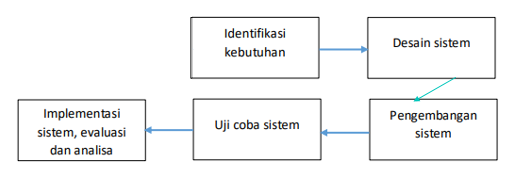
\includegraphics[scale=0.45]{gambar/Screenshot 2023-06-10 193529.png}
  % Keterangan gambar yang diinputkan
  \caption{Metodologi Penelitian}
  % Label referensi dari gambar yang diinputkan
  \label{fig:Metodologi}
\end{figure}

% Contoh penggunaan referensi dari gambar yang diinputkan
Gambar \ref{fig:Metodologi} menjelaskan tentang metodologi penelitian.

\section{Bahan dan peralatan yang digunakan}
Dalam penelitian ini, digunakan bahan dan peralatan yang dibutuhkan.
\subsection {Perangkat keras (hardware)}
Perangkat keras yang digunakan adalah sebagai berikut.
\begin{itemize}
 \item Laptop
 \item Mikrokontroler ESP32
 \item \emph{Webcam}
\end{itemize}

\subsection {Perangkat lunak (software)}
Perangkat lunak yang digunakan adalah sebagai berikut.
\begin{itemize}
 \item Arduino IDE
 \item Visual Studio Code
 \item GitHub
\end{itemize}


\section{Urutan pelaksanaan penelitian}

% Ubah tabel berikut sesuai dengan isi dari rencana kerja
\newcommand{\w}{}
\newcommand{\G}{\cellcolor{gray}}
\begin{table}[H]
  \captionof{table}{Tabel timeline}
  \label{tbl:timeline}
  \begin{tabular}{|p{3.5cm}|c|c|c|c|c|c|c|c|c|c|c|c|c|c|c|c|}

    \hline
    \multirow{2}{*}{Kegiatan} & \multicolumn{16}{|c|}{Minggu}                                                                       \\
    \cline{2-17}              &
    1                         & 2                             & 3  & 4  & 5  & 6  & 7  & 8  & 9  & 10 & 11 & 12 & 13 & 14 & 15 & 16 \\
    \hline

    % Gunakan \G untuk mengisi sel dan \w untuk mengosongkan sel
    Pengambilan data          &
    \G                        & \G                            & \G & \G & \w & \w & \w & \w & \w & \w & \w & \w & \w & \w & \w & \w \\
    \hline

    Pengolahan data           &
    \w                        & \w                            & \w & \w & \G & \G & \G & \G & \w & \w & \w & \w & \w & \w & \w & \w \\
    \hline

    Analisa data              &
    \w                        & \w                            & \w & \w & \w & \w & \w & \w & \G & \G & \G & \G & \w & \w & \w & \w \\
    \hline

    Evaluasi penelitian       &
    \w                        & \w                            & \w & \w & \w & \w & \w & \w & \w & \w & \w & \w & \G & \G & \G & \G \\
    \hline
  \end{tabular}
\end{table}



  \cleardoublepage

  % Konten lainnya
  % \chapter{HASIL YANG DIHARAPKAN}

\section{Hasil yang Diharapkan dari Penelitian}

Dari penelitian yang akan dilakukan, diharapkan alat yang dikembangkan berhasil dan dapat digunakan untuk mendeteksi ketersediaan ruang secara otomatis berdasarkan okupansi. 
Alat yang dibuat berukuran kecil, dan memiliki harga yang ekonomis


\section{Hasil Pendahuluan}

Sampai saat ini, kami telah \lipsum[16]

  % \cleardoublepage

  % Daftar pustaka
  % Daftar pustaka
\chapter*{DAFTAR PUSTAKA}
\addcontentsline{toc}{chapter}{DAFTAR PUSTAKA}
\renewcommand\refname{}
\vspace{2ex}
\renewcommand{\bibname}{}
\begingroup
\def\chapter*1{}
\printbibliography
\endgroup
\cleardoublepage

\end{document}